\section{Typed realizability}
\label{sec:typed-realizability}

RZ is based on \emph{typed realizability} by John
Longley~\cite{Longley99}. It is a variant of realizability that most
directly corresponds to the informal view that a programmer has in
mind when thinking about an implementation of a structure.

We motivate and explain typed realizability and its relationship with
real-world programming by way of example. Suppose we are asked to
design a data structure for the set $\mathcal{G}$ of all finite
simple\footnote{There is at most one arrow between any two vertices.}
directed graphs with vertices labelled by integers. An exemplar
directed graph~$G$ is shown in Figure~\ref{fig:digraph}.
%
\begin{figure}
  \centering
  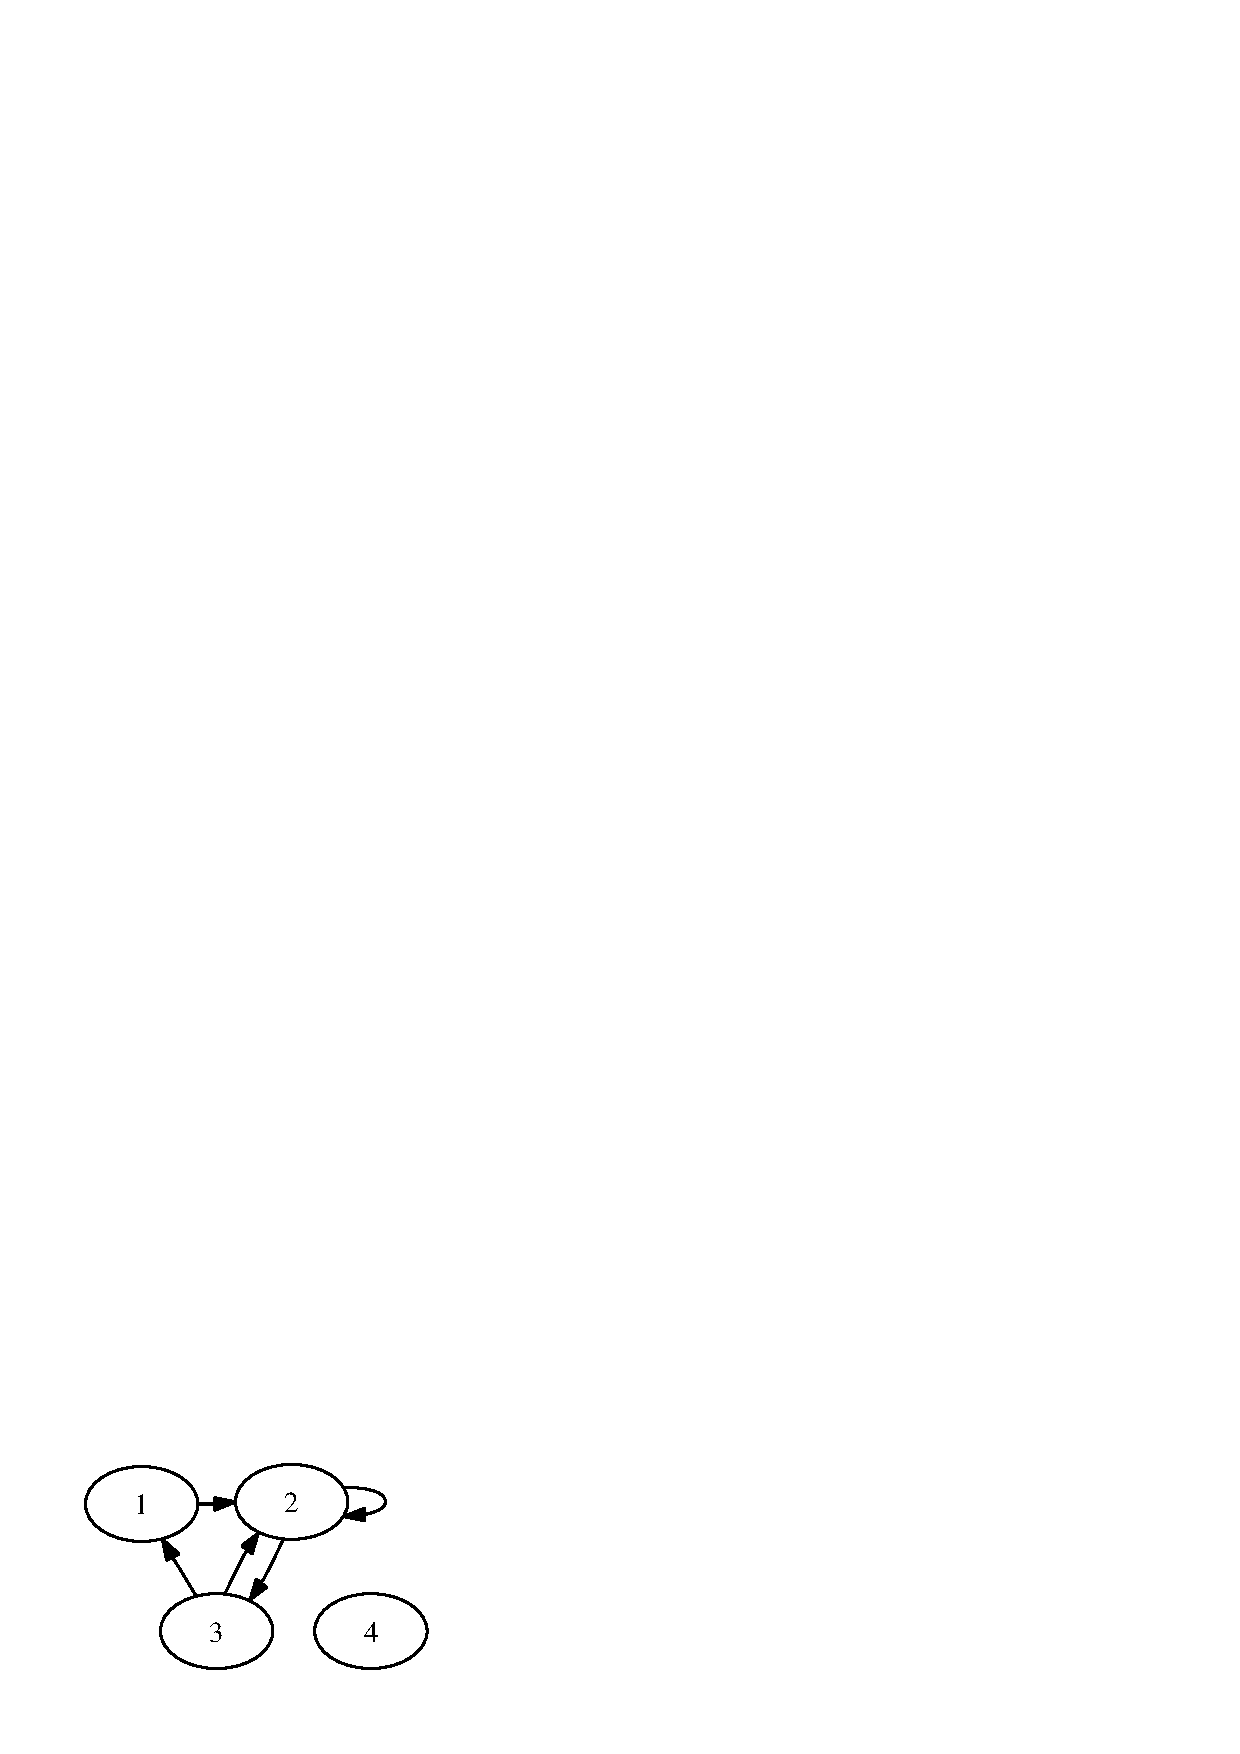
\includegraphics[width=0.4\textwidth]{digraph}
  \caption{A finite directed graph $G$}
  \label{fig:digraph}
\end{figure}
%
A common representation is a pair of lists $(\ell_V, \ell_A)$, where
$\ell_V$ is the list of vertices and $\ell_A$ the list of arrows,
known as the \emph{adjacency list}. In our example, $\ell_V = [1; 2;
3; 4]$ and $\ell_A = [(1,2); (2,2); (2,3); (3,2); (3;1)]$. Thus we
define the datatype of graphs to be\footnote{We use Ocaml notation in
  which $\clist{t}$ means lists of elements of type~$t$, and
  $t_1 * t_2$ means the type of ordered pairs whose first component
  has type $t_1$ and second type $t_2$.}
%
\begin{equation*}
  \ctype \mathtt{graph} = \clist{\cint} * \clist{(\cint * \cint)}
\end{equation*}
%
However, this is not a complete description of the representation, as
there are invariants and conditions which are not expressed directly
in the programming language, such as:
%
\begin{enumerate}
\item The order in which vertices and arrows are listed is not
  important, e.g., $[1;2;3;4]$ and $[4;1;2;3]$ represent the same vertices.
\item Each vertex and arrow must be listed exactly once.
\item Infinite, cyclic lists, and non-terminating expressions are not
  valid representations, e.g.,
  %
  \begin{equation*}
    \cwhile{\ctrue}{()}; [(1,2);(2,2);(2,3);(3,2);(3;1)]
  \end{equation*}
  %
  is not a valid adjacency list, and neither is an expression that
  raises an exception.
\item We ought to decide which computational effects, if any, are
  allowed, e.g., is
  %
  \begin{equation*}
    \cprint{\cstring{Hello}}; [(1,2);(2,2);(2,3);(3,2);(3;1)]
  \end{equation*}
  %
  a valid adjacency list?
\end{enumerate}
%
To summarize, an implementation of the set~$\mathcal{G}$ should tell
us not only what the underlying datatype $\mathtt{graph}$ is, but also
which values of type $\mathtt{graph}$ represent which elements
of~$\mathcal{G}$. As we shall see next, all of this can be expressed
either as a \emph{realizability relation} or a \emph{partial
  equivalence relation (per)}.


\subsection{Modest sets and pers}
\label{sec:modest-sets-pers}

We now give the formal definition of typed realizability, as it
applies to Ocaml. Other general-purpose programming languages could be
used instead, as long as they provide the usual ground types, product
and function types. Additionally, it is convenient to work with a
language that supports sum types, as this allows a more natural
representation of disjoint unions.

Let $\Type$ be the collection of all (non-parametric) Ocaml types. To
each type $t \in \Type$ we assign the set $\values{t}$ of values of
type~$t$ which behave \emph{functionally} in the sense
of~\cite{longley99when}. Such values are represented by terminating
expressions which do not raise exceptions or return different results
on different invocations, although they \emph{may} use exceptions,
store, and other computational effects, as long as they behave as if
they did not. A useful example of a functional value using store is
presented in Section~\ref{sec:we-show-modulus-of-continuity-example}.
Note also that a functional value of a functional type may diverge as
soon as it is applied, e.g., if we define
$\cletrec{f\;(x:\cint):\cint}{f\;x}$ then $f \in \values{\cint \to
  \cint}$. The collection $\Type$ with the assignment of functional
values $|t|$ to each $t \in \Type$ forms a \emph{typed partial
  combinatory algebra (TPCA)}, which provides a theoretical basis for
the definition of a realizability model that suits our needs.

Going back to our example, we see that to implement the set of
directed graphs $\mathcal{G}$ is to specify a datatype
$\typeOf{\mathcal{G}} = \mathtt{graph}$ together with a
\emph{realizability relation} $\rz_{\mathcal{G}}$ between
$\mathcal{G}$ and $\values{\mathtt{graph}}$. The meaning of $(\ell_V,
\ell_A) \rz_\mathcal{G} G$ is ``value $(\ell_V, \ell_A)$ represents
(realizes, implements) graph $G$''. There are two natural conditions
that $\rz_\mathcal{G}$ ought to satisfy: (1) for every $G \in
\mathcal{G}$ there should be at least one realizer $(\ell_V, \ell_A)$
representing it, and (2) if $(\ell_V, \ell_A)$ represents both $G$ and
$G'$ then $G = G'$. The latter condition is called \emph{modesty} and
is not strictly necessary for the development of the theory, though it
is something that programmers would naturally expect to hold. If
$(\ell_V, \ell_A)$ and $(\ell'_V, \ell'_A)$ represent the same graph,
we say that they are \emph{equivalent} and write $(\ell_V, \ell_A)
\per_\mathcal{G} (\ell'_V, \ell'_A)$. The relation $\per_\mathcal{G}$
is a \emph{partial} equivalence relation (symmetric and transitive,
but not reflexive) because not every $(\ell_V, \ell_A) \in
\values{\mathtt{graph}}$ represents a graph.

\bigskip

A general definition is in order. A \emph{modest set} is a triple $A =
(\setOf{A}, \typeOf{A}, {\rz_A})$ where $\setOf{A}$ is the
\emph{underlying set}, $\typeOf{A} \in \Type$ is the \emph{underlying
  type}, and $\rz_A$ is a \emph{realizability relation} between
$\values{\typeOf{A}}$ and $\setOf{A}$, satisfying
% 
\begin{enumerate}
\item \emph{totality:} for every $x \in \setOf{A}$ there is $v \in
  \typeOf{A}$ such that $v \rz_A x$, and
\item \emph{modesty:} if $u \rz_A x$ and $u \rz_A y$ then $x = y$.
\end{enumerate}
%
The \emph{support} of $A$ is the set $\support{A} = \set{v \in
  \typeOf{A} \such \xsome{x}{\setOf{A}}{v \rz_A x}}$ of those values
which realize something. We define the relation $\per_A$ on
$\values{\typeOf{A}}$ by
%
\begin{equation*}
  u \per_A v
  \iff
  \some{x}{\setOf{A}}{u \rz_A x \land v \rz_A x} \;.
\end{equation*}
%
From totality and modesty of $\rz_A$ it follows that $\rz_A$ is a per,
i.e., symmetric and transitive. Observe that $\support{A} = \set{v \in
  \values{\typeOf{A}} \such v \per_A v}$, whence $\per_A$
restricted to $\support{A}$ is an equivalence relation. In fact, we
may recover a modest set up to isomorphism from $\typeOf{A}$ and
$\per_A$ by taking $\setOf{A}$ to be the set of equivalence classes of
$\per_A$, and $v \rz_A x$ to mean $v \in x$.

The two views of implementations, as modest sets $(\setOf{A},
\typeOf{A}, {\rz_A})$, and as pers $(\typeOf{A}, {\per_A})$, are
equivalent. In RZ we use pers because they refer only to types and
values, as opposed to arbitrary sets. Nevertheless, it is useful to
understand how modest sets and pers arise from natural considerations
about programming practice.

Modest sets form a category whose objects are modest sets and
morphisms are the realized functions. A \emph{realized function} $f :
A \to B$ is a function $f : \setOf{A} \to \setOf{B}$ for which that there
exists $v \in \values{\typeOf{A} \to \typeOf{B}}$ such that, for all
$x \in \setOf{A}$ and $u \in \typeOf{A}$,
%
\begin{equation}
  \label{eq:rz-function-space}
  u \rz_A x \implies v\;u \rz_B f(x) \;.
\end{equation}
%
This condition is just a mathematical expression of the usual idea
that~$v$ is an implementation of~$f$, since~$v$ does to realizers
what~$f$ does to the elements they represent.

The equivalent category of pers has as objects pairs $A = (\typeOf{A},
{\per_A})$ where $\typeOf{A} \in \Type$ and $\per_A$ is a per on
$\values{\typeOf{A}}$. A morphism $A \to B$ is represented by $v
\in \values{\typeOf{A} \to \typeOf{B}}$ such that, for all $u, u'
\in \support{A}$,
%
\begin{equation}
  \label{eq:per-exponential}
  u \per_A u' \implies v\;u \per_B v\;u' \;.
\end{equation}
%
Values $v$ and $v'$ which both satisfy~\eqref{eq:per-exponential}
represent the same morphism if, for all $u, u' \in \support{A}$,
%
\begin{equation*}
  u \per_A u' \implies v\;u \per_B v'\;u' \;.
\end{equation*}

The category of modest sets has a very rich structure. For example, we
may form a cartesian product $A \times B$ of modest sets $A$ and $B$
by
%
\begin{align*}
  \setOf{A \times B} &= \setOf{A} \times \setOf{B},\\
  \typeOf{A \times B} &= \typeOf{A} * \typeOf{B},\\
  p \rz_{A \times B} (x,y) &\iff
  \cfst{p} \rz_A x \land \csnd{p} \rz_B y.
\end{align*}
%
The projections $\pi_1 : A \times B \to A$ and $\pi_2 : A \times B \to
B$ are realized by $\mathtt{fst}$ and $\mathtt{snd}$, respectively.

The morphisms between modest sets~$A$ and~$B$ again form a modest set
$B^A$, also written as $A \to B$, called the \emph{exponential} of~$A$
and~$B$, with the underlying set
%
\begin{equation*}
  \setOf{B^A} =
  \set{f : \setOf{A} \to \setOf{B} \such \text{$f$ is a realized function}},
\end{equation*}
%
the underlying type
%
\begin{equation*}
  \typeOf{B^A} = \typeOf{A} \to \typeOf{B},
\end{equation*}
%
and the realizability relation $\rz_{B^A}$ defined
by~\eqref{eq:rz-function-space}. The evaluation map $e : B^A \times A
\to B$, $e(f,x) = f(x)$ is realized by Ocaml application,
$\cfun{(u,v)}{u\;v}$. If a function $f : C \times A \to B$ is realized
by $v$, then its transpose $\tilde{f} : C \to B^A$, $\tilde{f}(z)(x) =
f(z,x)$, is realized by $\cfun{z\;x}{v \; (z,x)}$. This shows that the
category of modest sets is cartesian closed. In
Section~\ref{sec:realizability-interpretation} we review other
canonical constructions on modest sets.

\bigskip

As an example we consider the cyclic group on seven elements $(\ZZ_7,
0, {-}, {+})$. To implement the group, we must give a representation
of $\ZZ_7$ as a modest set~$Z = (\ZZ_7, \typeOf{Z}, {\rz_Z})$, provide
a realizer for the neutral element~$0$, and show that negation~$-$ and
addition~$+$ are realized. We represent the elements of~$\ZZ_7 =
\set{0, 1, \ldots, 6}$ with values of type $\typeOf{Z} = \cint$. We
allow any integer $v \in \values{\cint}$ to represent the element $v
\mathbin{\mathrm{mod}} 7$,
%
\begin{equation*}
  v \rz_Z k \iff v \mathbin{\mathrm{mod}} 7 = k \;.
\end{equation*}
%
The neutral elements $0$ is represented by~$0$, while negation and
addition are implemented by
%
\begin{align*}
  &\clet{\mathtt{neg}\; k}{-(k \cmod 7)} \\
  &\clet{\mathtt{add}\; k\; m}{(k \cmod 7) + (m \cmod 7)}
\end{align*}
%
The expected $\clet{\mathtt{neg}\; k}{-k}$ and $\clet{\mathtt{add}\;
  k\; m}{k+m}$ do not work because of overflow at values that exceed
$2^{30}$ (on a 32-bit machine). (We could avoid the overflow worries
by taking an isomorphic representation in which the only valid
realizers are $0$, $1$, \ldots, $6$, and negation and addition
realized by $\clet{\mathtt{neg}\; k}{7 - k}$ and $\clet{\mathtt{add}\;
  k\; m}{(k + m) \cmod 7}$, respectively.)

The modest set~$Z$ also has \emph{decidable equality}, which means
that the characteristic map $\mathrm{eq} : Z \times Z \to
\set{\mathtt{false}, \mathtt{true}}$ of equality is realized, namely
by\footnote{Incidentally, $\cfun{(k,m)}{(k - m) \cmod 7 = 0}$ does not
  decide equality because of possible overflow in subtraction, whereas
  $\cfun{(k,m)}{k \cmod 7 = m \cmod 7}$ does not work because in Ocaml
  $a \cmod b$ is negative when~$a$ is negative, e.g., $(-10) \cmod 7 =
  -3$ instead of the expected $4$.} $\cfun{(k,m)}{(k \cmod 7 - m \cmod
  7) \cmod 7 = 0}$. However, not all modest sets have decidable
equality, since there may not be a decision procedure for determining
whether two realizers represent the same element. In particular, this
would happen if we implemented a semigroup with an undecidable word
problem~\cite{post47:_recur_unsol_probl_thue}.


\subsection{Uniform families of modest sets}
\label{sec:uniform-families}

Many structures are naturally viewed as families of sets, or sets
depending on parameters, or \emph{dependent types} as they are called
in type theory. For example, the $n$-dimensional Euclidean space
$\RR^n$ depends on the dimension $n \in \NN$, the Banach space
$\mathcal{C}([a,b])$ of uniformly continuous real functions on the
closed interval $[a,b]$ depends on $a, b \in \RR$ such that $a < b$,
etc. In general, a family of sets $\family{A_i}{i \in I}$ is an
assignment of a set $A_i$ to each $i \in I$ from an \emph{index
  set}~$I$.

In the category of modest sets the appropriate notion is that of a
\emph{uniform} family~$\family{A_i}{i \in I}$, which is an assignment
of a modest set $A_i = (\setOf{A_i}, \typeOf{A}, {\rz_{A_i}})$ to each
$i \in \setOf{I}$, where $I$ is an index modest set,
cf.~\cite{Jacobs,Birkedal}. The uniformity comes from the requirement
that all the~$A_i$'s share the same underlying type~$\typeOf{A_i} =
\typeOf{A}$. It is a desirable restriction from the implementation
point of view, because it removes dependencies at the level of types.
Note also that there is no dependency on the realizers, only on the
elements of the underlying set.

We may form the \emph{sum} $\depsum{i \in I}{A_i}$ of a uniform family
$\family{A_i}{i \in I}$ as
%
\begin{align*}
  \setOf{\depsum{i \in I}{A_i}} &=
  \set{\pair{i,x} \such i \in \setOf{I} \land x \in \setOf{A_i}}
  \\
  \typeOf{\depsum{i \in I}{A_i}} &=
  \typeOf{I} \times \typeOf{A}
  \\
  (u,v) \rz_{\depsum{i \in I}{A_i}} (i,x)
  &\iff
  u \rz_I i \land v \rz_{A_i} x
\end{align*}
%
and the \emph{product} $\depprod{i \in I}{A_i}$ as
%
\begin{align*}
  \setOf{\depprod{i \in I}{A_i}} &=
  \set{f : \setOf{I} \to {\textstyle \bigcup_{i \in \setOf{I}} \setOf{A_i}} \such
    \xall{i}{\setOf{i}}{f(i) \in \setOf{A_i}}}
  \\
  \typeOf{\depprod{i \in I}{A_i}} &=
  \typeOf{I} \to \typeOf{A}
  \\
  u \rz_{\depprod{i \in I}{A_i}} f
  &\iff
  \xall{i}{I}{\all{v}{\typeOf{I}}{
      v \rz_I i \implies
      u \; v \rz_{A_i} f(i)
    }}.
\end{align*}
%
These constructions allow us to interpret (extensional) dependent type
theory in the category of modest sets.

As an example of a uniform family we consider the cyclic group
$(\ZZ_n, 0, {-}, {+})$ of order $n$. Essentially, we just replace~$7$
by~$n$ everywhere in the above example:
%
\begin{align*}
  & \setOf{Z_n} = \ZZ_n = \set{0, 1, \ldots, n - 1}
  \\
  & \typeOf{Z_n} = \cint
  \\
  & v \rz_{Z_n} k \iff v \mathbin{\mathrm{mod}} n = k
  \\
  & \clet{\mathtt{neg}\; k }{- (k \cmod n)}
  \\
  & \clet{\mathtt{add}\; k \; m}{k \cmod n + m \cmod n}.
\end{align*}
%
These definitions make sense for $n \geq 1$, but for too large a value
of~$n$ overflow might occur. If we expect the implementation to be
used with such values, it is more prudent to replace the type~$\cint$
with an implementation of arbitrary size integers.

\internal{Andrej}{I have set up this example so that it looks ok, but
  it actually incomplete because we have not specified the index
  modest sets. Maybe we can use this later on. If not, I'll include
  the definition of the index modest set.}

%%% Local Variables: 
%%% mode: latex
%%% TeX-master: "cie"
%%% End: 
